
\subsection{Fundamental Matrix}

In order to describe this technique, linear algebra is used. Firstly, all of the transforms required to represent imaging systems can be represented using $4 \times 4$ matrices and homogeneous vectors (with four rows and a single column). These important transforms include: 3D rotation, scaling, shearing/skewing, mirroring, translation and perspective. Rather than describing camera capture using projecting rays, we can use linear algebra which provides further capabilities and allows us to estimate the fundamental matrix. 

In figure \ref{fig:INTRO_FMA1} there are two camera systems, for this part of the discussion we focus on the left camera $C_{1}$ and the left frame. Next we will describe how point $Q$ is projected from 3D onto the 2D point $Q_{1}$. First, $C_{1}$ is translated to the origin (later this allows rotation and perspective transforms to more easily be performed). In order to do this, $C_{1}$ can be subtracted from itself (to become the origin) and so it is also subtracted from $Q$ as well. Rather than performing this directly though, we will use a $4 \times 4$ translation matrix T instead. Next, rotation is performed in order to align the camera's axes with the x, y and z axes. The camera's axes can be defined using three vectors. One pointing directly ahead where the camera is facing (piercing the center of the projection frame), another points directly to the right perpendicularly (orthogonal to the first), the final points above the camera, aligned orthogonally with the previous two vectors. \\

These three axes can be placed into the columns of a four by four homogeneous matrix. This forms a matrix which rotates an aligned camera's axes to face the direction where $C_1$ currently points to. In other words, it performs the exact opposite of what is needed. Since this matrix is orthogonal (known because the column vectors are all perpendicular) the inverse transform is simply the transpose of this matrix. This rotation matrix will be named R. Next, there may be a lateral alignment, this is a translation which further aligns the points to the center of the frame. This is performed using another $4 \times 4$ matrix, L. Finally, another $4 \times 4$ matrix, P is used to project the point $Q$ to the 2D point, $Q_1$. The entire projection can be performed by multiplying these matrices together, $Projection = P * L * R * T$. Here, $P * L$ are known as the intrinsic parameters whilst $R * T$ are called the extrinsic parameters. Due to the imperfect nature of the camera lens, the intrinsic camera matrix often has distortion, this becomes important later when we define the difference between the fundamental matrix and another matrix introduced, the essential matrix.

\begin{figure*}[t!]
	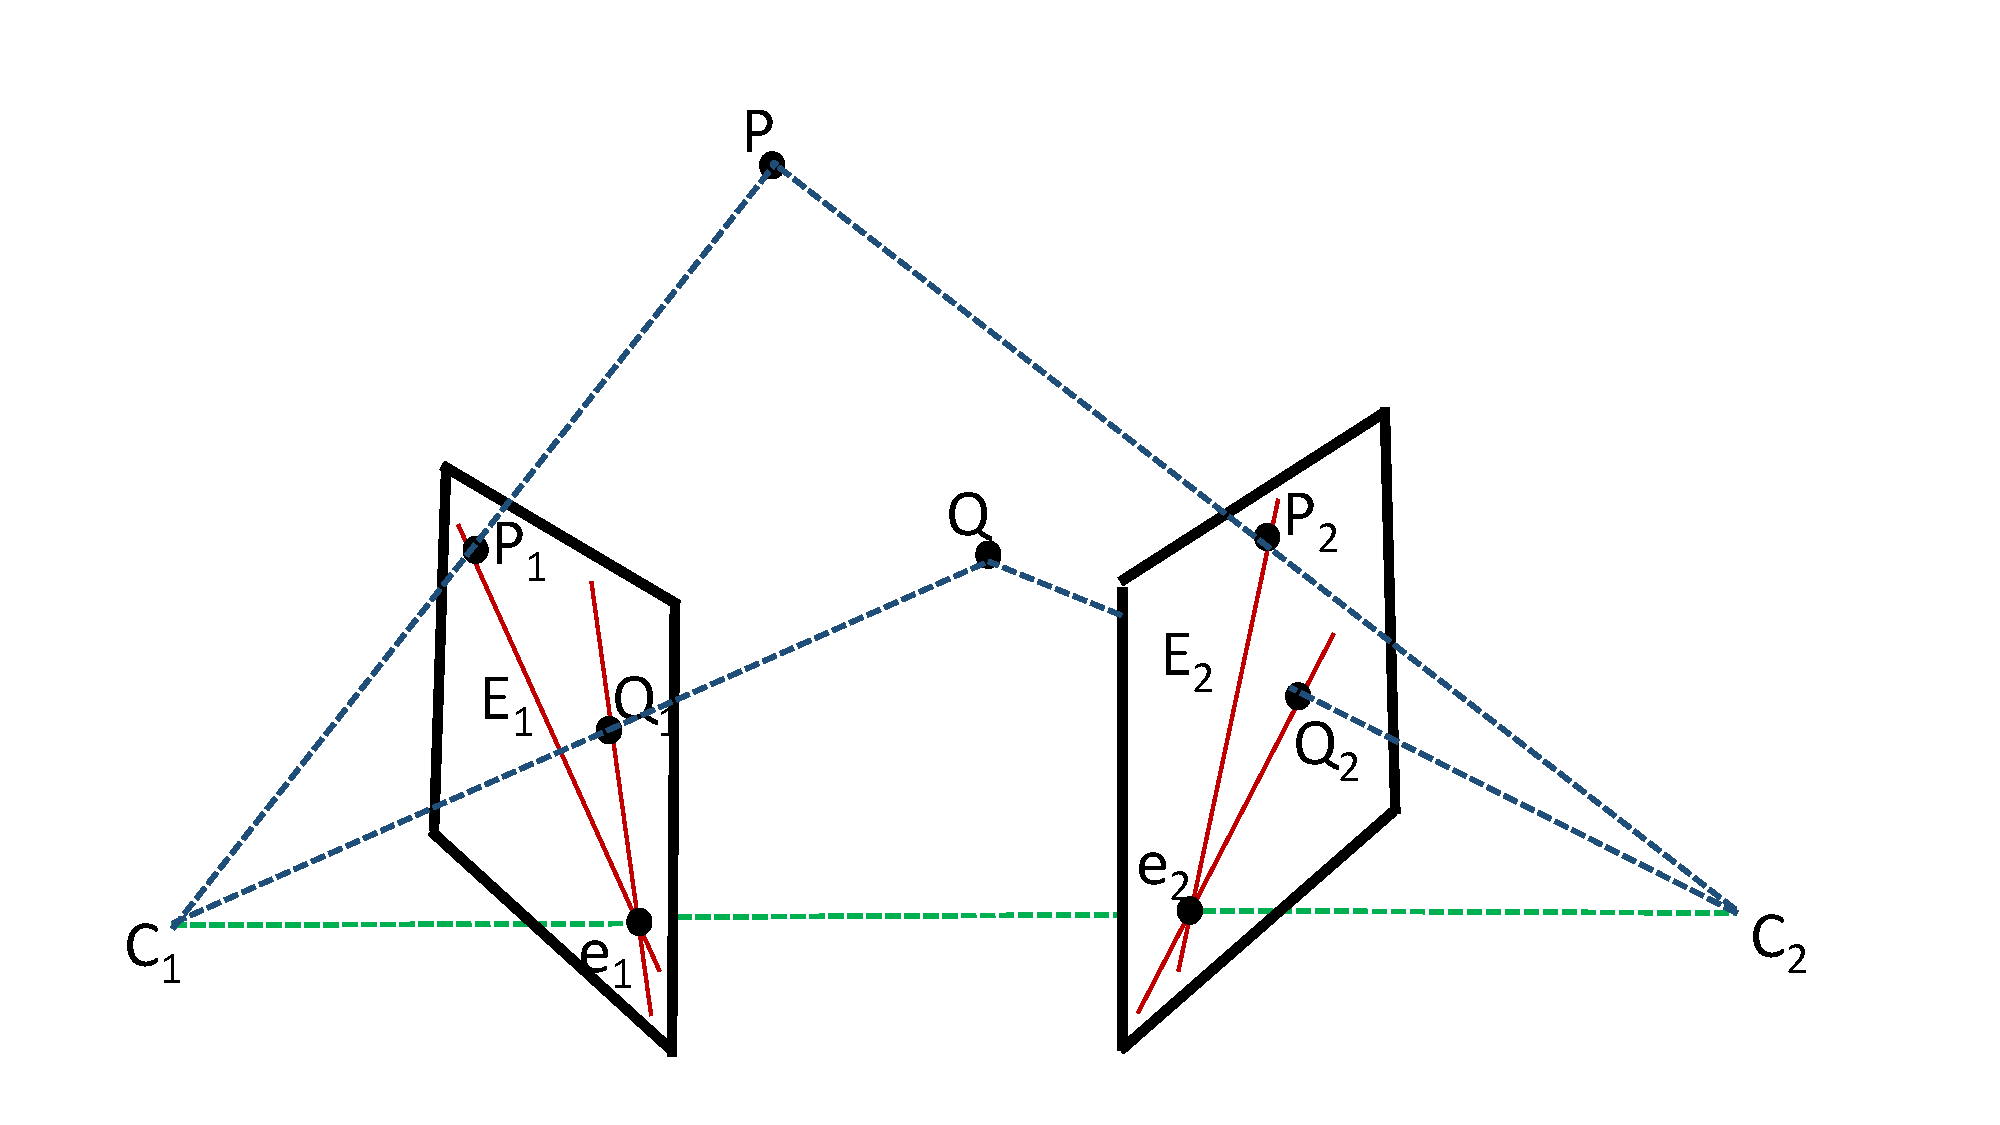
\includegraphics[width=5.0in]{images/introfm1}
	\caption{A pair of cameras viewing two points. This figure is a reconstruction of the figure on page 492 in Computer and machine vision: theory, algorithms, practicalities \cite{Davies12Computer}.}
	\label{fig:INTRO_FMA1}
\end{figure*}  

Using the steps described and looking at figure \ref{fig:INTRO_FMA1}, we now know how 3D point $P$ can be mapped to both of the frames with cameras $C_1$ and $C_2$. Projecting point $P$ onto the two frames gives points $P_1$ and $P_2$ respectively. Next, we describe the relation between vectors, $V_1$, formed by normalising the vector from $C_1$ to $P$, and $V_2$ (normalizing $(P - C_1)$. Skipping past the mathematical proof, which is detailed in Computer and Machine Vision \cite{Davies12Computer}, the relation between between these vectors is the essential matrix, $E$. This relation is $V_2^{T} * E * V_1 = 0$. Unfortunately we may not know the depth of $P$ and unless an investigation is performed on the particular camera system in use, we do not know the precise perspective transform and associated distortion. Fortunately, both the depth and the perspective are cancelled in this matrix formulation, and so we can specify the relation using only the 2D points, $P_1^T * E * P_2 = 0$. \\

This formula is based on the assumption that no distortion present in the camera system. In this case, both of the cameras may have distortion. We represent this distortion here using matrices $G_1$ and $G_2$. If both shots are taken with the same camera, we may assume $G_1 = G_2$. We therefore relate the theoretically precise $P_1$ and $P_2$ with their real world equivalents (which have distortion) $D_1$ and $D_2$ by $P_1 = Q_1^{-1} * D_1$ and $P_2 = Q_2^{-1} * D_2$. Inserting this into the essential matrix formulation we have, $(Q_1^{-1} * D_1)^T * E * Q_2^{-1} * D_2 = D_{1}^{T} * {Q_1^{-1}}^{T} * E * Q_2^{-1} * D_2 = 0$. The presence of this distortion is the difference between the essential and fundamental matrices with the fundamental matrix being $F = {Q_1^{-1}}^{T} * E * Q_2^{-1}$. If no distortion is present, the fundamental matrix is equivalent to the essential matrix. \\

Looking at figure \ref{fig:INTRO_FMA1} again, line $E_1$ represents something called an epipolar line, this line lies on the plane in which both cameras and point $P$ sit on. Line $E_1$ is the epipolar line of the left frame and $E_2$ is the epipolar line of the right frame. Point $e_1$ is the epipole of the left frame and point $e_2$ is the epipole of the right frame. Epipoles are the projection of one camera's location onto the frame of another camera. The projection of $C_2$ onto the left frame by camera $C_1$ is the epipole $e_1$. If the fundamental matrix is multiplied by a particular point it produces a vector in $R^3$ which represents the epipolar line as $[a b c]^T$ in which $a,b$ and $c$ represent the line equation $ax^2 + bx + c$. We can see that the epipolar line corresponding to $Q$ and $Q_1$ passes through a common point with the other epipolar line $E_1$. In fact, all epipolar lines intersect at the epipole. Therefore, if the fundamental matrix can be computed, so can the epipolar lines and the epipoles. \\

The fundamental matrix can be computed using around 8 point matches between images. Using the fundamental matrix, image rectification can be performed as well as 3D reconstruction. Using point $P$ in figure \ref{fig:INTRO_FMA1}, we already know the fundamental matrix, epipolar lines and epipoles can be computed from the point correspondences. If the epipoles are known, then we know the direction in which the other camera resides, in that case, all that is left is to triangulate the point correspondences in order to solve for the extrinsic camera parameters. The basic pipeline for the fundamental matrix method begins with feature matching, followed by fundamental matrix estimation. Then the extrinsic camera information is estimated and images are rectified and so that disparity information can be computed. Then depth maps can be projected through any of the two cameras and aligned. \\


Monocular Feature based SLAM systems use feature matches to estimate camera pose and location changes across frames \cite{Davison02Simultaneous}. Variations of this method use different features including: corners and lines \cite{Jeong06Visual}, image patches \cite{Silveira08Efficient} and exemplar feature matching \cite{Chekhlov07Robust}. SIFT features are used most often in SLAM \cite{Jensfelt06Framework,Pollefeys08Detailed,Beall11Bundle,Eudes10Fast}, in addition FAST features have been explored \cite{Kundu10Realtime,Leelasawassuk133d,Konolige10View,Konolige08Frameslam}. Beall et al \cite{Beall11Bundle} made use of both SIFT and SURF features in their underwater SLAM system. Real-time monocular SLAM systems based on this approach have also been proposed \cite{Chekhlov07Robust,Pollefeys08Detailed}. RANSAC is often used in monocular SLAM \cite{Eudes10Fast,Kundu10Realtime,Konolige10View,Konolige08Frameslam,Pradeep13Monofusion} to remove outliers which cause incorrect camera parameter estimates. Bundle adjustment is also used as an additional step to refine camera parameter estimation \cite{Eudes10Fast}. 


in monocular setting, the scale of the map cannot be  determined \cite{Endres12Evaluation}

SLAM has focused on real time markerless tracking and live scene reconstruction based on a single sensor RGB eg. MonoSLAM[8] \cite{Davison03Real} which is less accurate than PTAM [17] \cite{Klein07Parallel}  but these only produce sparse reconstructions
some methods have grown to combine PTAM's camera tracking ability with MVS-style reconstructions [19/26] (\cite{Newcombe10Live}/\cite{Stuhmer10Real})
recently: iterative image alignment has been used to replace features in tracking [20] \cite{Newcombe11Dtam}
this scene is promising: but monocular based dense 3D reconstruction is difficult and requires suitable camera motion and scene illumination


\subsection{Stereo based}

Stereo based SLAM systems also use features to estimate camera parameters. However, stereo based systems are capable of generating dense depth data more easily using stereo algorithms. Miro et al \cite{Miro06Towards} proposed a stereo based method which uses SIFT and the extended Kalman filter. The method by Van Gool et al \cite{Pollefeys04Visual} works with un-calibrated stereo pairs. It uses Harris corner features and a multi-view stereo algorithm. Sim et al \cite{Sim05Vision} and Gil et al \cite{Gil06Improving} both presented stereo based SLAM systems which use SIFT.

\cite{Endres12Evaluation}(
in monocular setting, the scale of the map cannot be  determined 
stereo slam [17 \cite{Konolige08Outdoor}, 24 \cite{Paz08Large}] -> does not suffer from this
only accurate for textured surfaces, non-textured surfaces cannot be estimated with depth );

SFM and MVS (multi view stereo) has given good results : camera tracking  and sparse reconstructions [10] \cite{Fitzgibbon98Automatic}, \cite{Seitz06Comparison} [24] 


[19 \cite{Newcombe10Live}] uses dense optical flow with PTAM like tracking for dense recon
this relies on camera poses coming from PTAM
[26 \cite{Stuhmer10Real}] do the same with near real time depth map calculation


\subsection{Feature Matching and RANSAC}

icp often not necessary and expensive
icp only used if no keypoint matches found... \cite{Endres12Evaluation}

The computation of pose without ICP, purely from feature matching is non-trivial because in reality, the system may suffer from the following:

\begin{itemize}
\item Synchronization problems between the RGB camera and Infrared camera shutters
\item depth jump interpolation - the interpolation of computed depth at object boundaries
\item feature matches often occur at depth jumps
\end{itemize}

RANSAC \cite{Fischler81Random} is able to deal with noisy data by filtering out points considered to be outliers.


\subsubsection{RGB-D SLAM}

Endres et al \cite{Endres12Evaluation} presented a dense 3D reconstruction technique using RGB-D data from the Kinect sensor based on feature matching and RANSAC. They also evaluated their technique under different illumination and camera movement speed conditions. It is able to operate at near real time speeds in small in-door environments. This method begins by feature matching RGB images across frames. Using the projected 3D points available for each pixel in the depth map, RANSAC \cite{Fischler81Random} is used to compute the camera pose across frames. These poses are optimized globally using the $g^2$o graph optimizer, the Octomap representation \cite{Wurm10Octomap} is used to voxelize the 3d points before storing them in a volumetric occupancy map. Since this system is based on feature matching, Endres et al evaluate 3 different feature matching techniques: SIFT \cite{Lowe04Distinctive} , SURF \cite{Bay06Surf,Bay08Speeded} and ORB \cite{Rublee11Orb}. ORB feature matching is tested because it is faster than SIFT and SURF with slightly less accuracy, the authors also evaluate a GPU implementation of SIFT \cite{Wu07Siftgpu}. Endres et al evaluate their algorithm using their own benchmark \cite{Sturm11Towards}. Results show it can handle up to 50 degrees of rotation per second, and speeds of up to 43 centimetres per second.  \\


This system is divided into a front-end and a back-end. The front-end performs feature detection, matching and sensor pose estimation via the RANSAC method whereas the back-end performs non-linear pose optimization using the $g^2o$ optimization procedure   and integrates these results into an occupancy grid based on the Octomap. A diagram of the combined front-end and back-end systems is given in figure \ref{Endres12EvaluationPipeline}. 


\begin{figure}[!h]
\centering
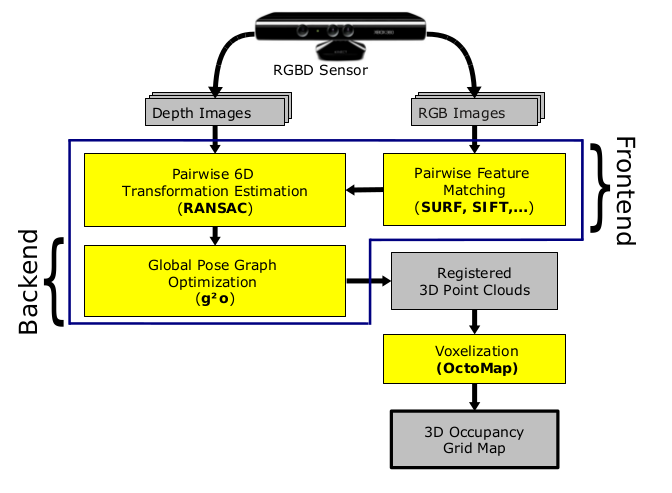
\includegraphics[width=12cm]{images/ch1/Endres12EvaluationPipeline}
\caption{RGB-D SLAM Pipeline used by Endres et al \cite{Endres12Evaluation}}
\label{Endres12EvaluationPipeline}
\end{figure}


The front-end uses OpenCV \cite{Bradski08Learning} for feature matching. During the feature detection process, the Hessian threshold is used to keep the total number of features constant. This is required because pose may not be able to be computed if there aren't enough features, but on the other hand, too many features typically lead to many false positives in the feature matching schema. As mentioned, these matched features (and thus matched 3d points) are used with RANSAC to compute pose \cite{Umeyama91Least}. During the RANSAC process, corresponding points with distances below 3cm are considered inliers. The inliers are then used exclusively to compute a finer pose. This method of pose estimation is fast but computational complexity depends on the number of features computed. For each frame, the pose relationship with 20 previous frames (including the most recent 3) is computed in parallel on the GPU. Then the final computed pose is given to the back-end. If accurate pose cannot be compute, constant motion is assumed. \\

comparable to the feature based rgb-d slam [8 \cite{Endres12Evaluation}]

\subsection{ICP}

icp[4 \cite{Besl92Method}]

(icp only minimizes error on point clouds, some other approaches minimize photometric error [20 \cite{Steinbrucker11Real}, 12 \cite{Kerl13Robust}] or combinations of both [23 \cite{Tykkala11Direct}]) -> these did not perform 3d reconstruction

6dof camera alignment and 3d surface reconstruction techniques developed in the graphics domain, here ICP is the most important
ICP @ [3 \cite{Besl92Method} ]
ICP is a non-linear optimization problem where approximations are found using the closest points currently for each
set
distance metrics have been researched using the point-plane metric [5 \cite{Chen92Object}]
[\cite{Chen92Object} 5] improves convergence rates, used for surface reconstructions which have normal data
computing closest points using ICP is expensive, there is projective data association algorithm [4 \cite{Blais95Registering}]
can be used for data in projective form (2d image where each image is a 3d point)
can reduce icp set to possible set of points or with a coarse to fine scheme
SLAM may use ICP to estimate camera changes





\subsubsection{Henry10Rgb}

henry [12 \cite{Henry10Rgb,Henry14Rgb}] is similar to this work \cite{Endres12Evaluation}
uses sparse keypoint matches between color images as initialization to icp
henry used sparse bundle adjustment [19 \cite{Lourakis09Sba} ], here 3d pose graph using [18 \cite{Kummerle11G}] framework is used
henry put resulting into surfel representation, here volumetric voxel representation is used [33], can be used for robot localization, path planning and navigation [13 \cite{Hornung10Humanoid}]

henry [9 \cite{Henry10Rgb}], applied graph slam to rgb-d data, using visual features + icp combo [8 \cite{Endres12Evaluation} ] also did a similar system, on benchmark [22 \cite{Sturm12Benchmark}]


[14 \cite{Henry10Rgb}] uses rgb-d with kinect by frame by frame icp : feature matching is used with graph optimization for loop closure and global consistency -> global fusion presents better performance



ICP [2 \cite{Besl92Method}, 26 \cite{Rusinkiewicz01Efficient}, 27 \cite{Segal09Generalized}]

\subsubsection{Kinect Fusion}

Newcombe et al \cite{Newcombe11Kinectfusion} proposed an accurate, real-time dense 3d reconstruction algorithm which works well on complex indoor environments. This algorithm computes relationships between depth map frames generated using the Microsoft Kinect \cite{Zhang12Microsoft} sensor. By aligning depth maps this method is capable of tracking both camera pose and location as well as generating dense 3d reconstructions. Only depth data is used in alignment computations thus, consequently because the Kinect is a structured light based depth sensor Kinect Fusion works under any lighting condition, including complete darkness. Since they use the Kinect and GPU (both considered commodity hardware these days) the technique may be considered inexpensive. \\

The method works by computing camera pose, transforming depth data by a computed pose (frame-by-frame) and fusing this data into a global surface volume. It uses a coarse to fine grain iterative closest point (ICP) algorithm to compute camera pose. During the ICP phase, the target points come from the entire globally matched previous frames. Therefore this method is considered global rather than frame-to-frame based. Such a method has direct advantages over frame-by-frame feature matching, since all data is used to compute pose. The downside, is that this method fails to find global solutions due to the nature of ICP. This may occur when some frames must be skipped due to motion blur, or the camera passing over surfaces which do not reflect infra-red light. \\

\begin{figure}[!h]
\centering
%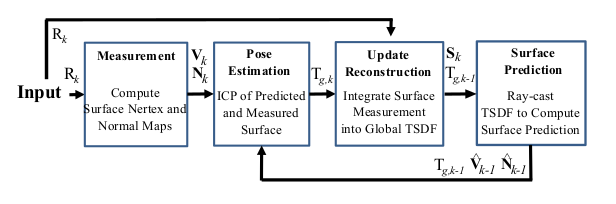
\includegraphics[width=12cm]{images/ch1/Newcombe11KinectFusion1}
\caption{Kinect Fusion Algorithm Pipeline \cite{Newcombe11Kinectfusion}}
\label{KFusionPipeliciteHne}
\end{figure}

Kinect Fusion has four main steps as illustrated in figure \ref{KFusionPipeline}. The first step named measurement, performs pre-processing on the depth data as well as generation of additional information for use by Kinect Fusion. Each depth map frame is first passed through a bilateral filter. From this, a dense vertex map (map of 3D points projected using a known projection matrix associated with the Kinect) is generated, as well as a normal map. For both the vertex and normal maps, a 3 level image pyramid is constructed. This makes the coarse to fine grain ICP technique possible. \\

Next, dense coarse to fine grain ICP is used to compute pose between the fused frames and the current frame. The authors exploit the fact that the transformation between frames is small because camera motion is slow when computing against every frame. With coarse-to-fine grain ICP they use projective data association \cite{Blais95Registering} and the point-plane metric for pose optimization \cite{Rusinkiewicz02Real}. The ICP based pose estimation computes pose given both a predicted and measured depth map. \\

After estimating camera pose relating to the globally fused model, each frame must be integrated into that model. The Kinect Fusion algorithm uses a truncated signed distance function (TSDF) representation. This is a signed distance function volume where the distances for each voxel are capped by some value. The TSDF uses a volume resolution of $512\times 512\times 512$. They use the TSDF, rather than relying on a linear but accurate discrete SDF transform \cite{Rasch09Remarks} because of the computational complexity of calculating the discrete SDF of large scale volumes. \\

As mentioned, Kinect fusion uses pose prediction and fuses each depth map into the TSDF representation. In this way, they align and fuse each depth map to the global 3d reconstruction. In this way, a global loop closure method is not required. This may have a negative side effect by which some frames which have larger resolutions may be heavily quantized in order to fuse with the SDF, especially very thin surfaces/objects. These features may also be advantageous for ICP in estimating pose. 


but kinect fusion generates synthetic depth images which are aligned to the current depth image using icp

newcombe [18 \cite{Newcombe11Kinectfusion} ] -> impressive results using sdfs to represent reconstruction, and icp for camera tracking

KF: for each image:
it renders a point cloud from the sdf at the previous pose using ray tracing and aligns this with the depth image



\subsection{Optimizers}

\subsubsection{3D Reconstruction by Optimizing directly in the SDF}

In 2013, Bylow et al \cite{Bylow13Real} presented a novel method which reconstructs static indoor environments in real time using RGB-D data captured using the Asus Xtion Pro Live sensor. Their system is able to generate accurate 3D RGB coloured models of the environment in real-time by optimizing for 6 degrees of freedom in terms of accurate projection of new depth map frames into an existing global signed distance function model of the scene. Their method uses several Gauss Newton optimization with a signed distance function representation, these techniques are represented and processed using a laptop with an NVIDIA GPU. Unlike Kinect Fusion \cite{Newcombe11Kinectfusion}, this method optimizes directly in the signed distance representation, in which camera pose is computed by finding a rotation and translation (6-DoF) which minimizes the error of projecting depth images into the SDF. Compared with the ICP based method used by Kinect Fusion, this technique is shown to be more robust and accurate. It compares favourably to bundle adjustment but is much faster for small to mid sized scenes. Results are generated using the TUM RGB-D benchmark and SDF volume sizes $256^3$ and $512^3$ are used in evaluations. The authors note the algorithm may be able to handle large scale scenes if used in conjunction with other techniques \cite{Kaess11Isam2,Kummerle11G}. \\

This technique is efficient because the error to minimize can be checked using several look-ups since the SDF itself contains the distances from each voxel to the global model's actual surface. Because of this, the algorithm is classified as working within global space rather than frame-by-frame. Using the SDF to lookup depth map projection error, the camera pose is iteratively estimated and then the depth map is integrated into the SDF and colour information is stored in another volume. The pose estimation procedure begins by storing the first frame as a volumetric signed distance function. Then for each new depth frame, camera pose is computed, and based on this pose the frame is projected into the scene. Using a lie algebra based 6-DoF model \cite{Ma12Invitation} envisioned as a vector in $R^6$ representing camera pose, the error for a given pose may be computed as the squared error of the depth map transformed by the pose and projected into the signed distance function. Due to noise or missing data within the depth frame, this error may never be reduced completely, instead the best pose is iteratively computed using this model and the Gauss Newton non-linear optimization algorithm. \\

The SDF representation uses two volumes as in \cite{Curless96Volumetric}, one volume stores the average distances, the other stores the cumulative weights for each voxel. Bylow et al use these weights to handle occlusion and sensor uncertainty. When integrating a point into the SDF, tri-linear interpolation is used between eight neighbours to handle point coordinated made up of floating point numbers. During integration, each voxel is projected onto the image plane rather than ray case from the center of projection as in \cite{Newcombe11Kinectfusion}. This ensures that each voxel is visited once when updating the SDF, whereas in the ray casting approach, this may not necessarily be the case. \\

In computing the SDF for a given depth map, the exhaustive marching cubes algorithm is too slow, even the fast marching algorithm \cite{Baerentzen01Implementation} is not suited for real time discrete SDF generation. Instead, the SDF is approximated with either the point to point distance or point to plane distance functions. For final visualization, marching cubes is used \cite{Lorensen87Marching} on the final SDF. Colour is computed from the colour volume using a technique found used by Whelan et al \cite{Whelan13Robust}. Since the method by Bylow et al is based on optimizing the projection error using the SDF and only uses locations in its pose estimation procedure, it is independent to illumination. Given this, it will also fail in cases where only co-planar surfaces are visible, they mention that using colour information during tracking \cite{Kerl13Robust} may mitigate these concerns.




\subsection{3D Features}

\cite{Aiger084}

4pcs - 4 points congruent sets for robust pairwise surface registration
fast and robust registration of wide base 3d data
resilient to noise and outliers
data can be raw, noisy and full of outliers
no need for pre-filtering or de-noising
significantly reduces the number of trials required to get registration, has no assumption of prior alignment
novel technique:
extracts all co-planar 4 points sets from a 3D point set which are approximately congruent under rigid transformation to a given set of co-planar 4-points
complexity O(n to power of 2 + k), n is number of points, k is number of 4 point sets
in practice: when not too much noise and overlap is significant,
using local descriptors allows for complexity O(n+k)
an extension to perform affine transforms too
demonstrates robustness over multiple range scans with varying levels of noise, outliers and overlap


methods of 3d alignment under rigid transformation with 3d scans
ns [\cite{Callieri04Roboscan} Callieri et al. 2004, Gelfand et al. 2005 \cite{Gelfand04Shape}, Li and Guskov
2005 \cite{Li05Multiscale}]

non-rigid alignments:
t [Pauly et al. 2005 \cite{Pauly05Example}, Brown and
Rusinkiewicz 2007 \cite{Brown07Global}].


local descriptor 3d features : ors [Li and Guskov 2005 \cite{Li05Multiscale}] can be used to define an approximate transformation, then use ICP to align further ([Besl and McKay 1992 \cite{Besl92Method}, Chen and Medioni 1992 \cite{Chen92Object}])

only need to know 3 point pairs

local descriptors (invariant to rigid transformations) can be used to extract these 3 points

geometric hashing may be used: [Wolfson and Rigoutsos 1997 \cite{Wolfson97Geometric}]

RANSAC can be used with the set of matches to find the best transform [Fischler and Bolles 1981 \cite{Fischler81Random}], 
these have been improved in by Chen and co-authors [1999] \cite{Chen99Ransac} which tradeoff speed for robustness

PCA can be used to compute bases but in the case of partial overlap, this quickly breaks down

local descriptors: [Johnson 1997 \cite{Johnson97Spin}, Li
and Guskov 2005 \cite{Li05Multiscale}],: 

under noisy conditions this may also be used : [Pottmann et al. 2007 \cite{Pottmann07Principal}],

an alternative is relying on the principal of large numbers
aka solving the largest common pointset (LCP) problem 
given point sets P and Q, LCP under δ-congruency solves for a subset Pi of P
having the largest cardinality such that the distance between T(Pi) and Q  is less than δ given an appropriate distance measure, given T is a rigid body transformation

the basic concept is to optimize the selection of the 3 points used as a base, choosing 3 then trying this out, then moving on,
this is O($m^3$ x $n^3$) but can be reduced to:  O($mn^3$ log n) [Irani and Raghavan \cite{Irani96Combinatorial} 1996] and even O($n^3$ log n) , but this is still expensive for large point sets

this paper introduces:
a novel 3d alignment scheme which does a rough alignment of surfaces which may have little overlap
this alignment may be refined using ICP  (cf. [Rusinkiewicz and Levoy 2001 \cite{Rusinkiewicz01Efficient}]). 

this method is based on the novel technique of extracting all co-planar 4 point from a 3D set that are related by rigid transform to a given planar 4-points in O($n^2$ + k) time

n is the number of points in Q and k is the number of 4-point sets

when simple reliable descriptors can be computed it is 
O(n+k)

can also be used to handle similarity transforms

bg
partial matching is fundamental task for registration and recognition of 3d objects [Frome et al 04 \cite{Frome04Recognizing}]

typically based on matching local descriptors [Jonson 1997 \cite{Johnson97Spin}, Mori \cite{Mori05Efficient} et al 05]

also integral invarients [Pottmann 07 \cite{Pottmann07Principal}]

can be used to accelerate 3d scans aquired by range scanners [Li and Gusov 05 \cite{Li05Multiscale}]

hough transform [ballard 97 \cite{Ballard81Generalizing}] ransac [fischler and bolles 81 \cite{Fischler81Random}]

image based alignment : [Wolfson and Rigoutsos \cite{Wolfson97Geometric} 97]

hashing based versions [Germain et al 97 \cite{Germain97Fingerprint}, Gal and Cohen-Or 06 \cite{Gal06Salient}, Mitra 06 \cite{Mitra04Registration}]

steps: pick a base P where the number of points in the base is equal to the number of points required to uniquely compute the transformation,

for each random base from Q, the corresponding alignment is vertified [Fischler and Bolles 81 \cite{Fischler81Random}, huttenlocher and ullman 90 \cite{Huttenlocher91Fast} ]

or voted for [Ballard 87 \cite{Ballard91Generalizing}]

variant of RANSAC , they use 4pcs for this step

finds all 4point sets from p and matches with all 4 points from Q

O($n^2$ + k) runtime to compute the 4 points


icp was too far to converge on a solution [Mitra et al 04 \cite{Mitra04Registration}]





